\documentclass[../Article_Design_of_Experiment.tex]{subfiles}
\graphicspath{{\subfix{../Figures/}}}
\begin{document}
			
	\subsubsection{Maximum likelihood}

	Following the work of \citet{Walter2010}, the vector $\hat{\Theta}_{ml}$ will be a maximum-likelihood estimate if it maximizes the cost function:
	
	{\footnotesize
	\begin{equation}
		j_{ml}(\Theta) = \pi_y (Y|\Theta) 
	\end{equation} }
	
	If $\Theta$ were fixed, $\pi_y(Y|\Theta)$ would be the probability density of the random vector $Y$ generated by a model with parameters $\Theta$ and observations $Y$. Considered as a function of $\Theta$, $\pi_y(Y|\Theta)$ is then called the likelihood of $Y$. The maximum-likelihood method looks for the parameter vector $\Theta$ value that gives the observed data the highest likelihood. In practice, it is often easier to look for $\hat{\Theta}_{ml}$ by maximizing the log-likelihood function, yielding the same estimate since the logarithm function is monotonically increasing.
	
	{\footnotesize
	\begin{equation}
		j_{ml}(\Theta) = \ln ( \pi_y (Y|\Theta) )
	\end{equation} }
	
	Assume that the observed outputs satisfy 
	
	{\footnotesize
	\begin{equation}
		Y(t_i) = y(t_i, \Theta^*) + \epsilon_i, \qquad i=1,...,n_t
	\end{equation} }
	
	where the vector $y(t_i, \Theta^*)$ is the output of a deterministic model, $\Theta^*$ is the true value of the parameter vector, and the error $\epsilon_i$ belongs to a sequence of independent random variables with probability density $\pi_{\epsilon}(\epsilon_i)$. Since the $\epsilon_i$ are independent
	
	{\footnotesize
	\begin{equation}
		\pi_{\epsilon}(\epsilon_1, \epsilon_2, ..., \epsilon_{n_t}) = \prod_{i=1}^{n_t} \pi_{\epsilon_i}(\epsilon_i)
	\end{equation} }
	
	Consider the output error
	
	{\footnotesize
	\begin{equation} \label{EQ:Error_measurment}
		e^y(t_i, \Theta) = Y(t_i) - y(t_i, \Theta)
	\end{equation} }
	
	For the true value of the parameters, it satisfies $e^y(t_i, \Theta^*)\\=\epsilon_i$. and, since $y$ is deterministic, $\pi_{y_i} (Y(t_i)|\Theta) = \pi_{\epsilon_i} (e^y(t_i),\Theta)$. The likelihood of the $n_t$ observations can be written as
	
	{\footnotesize
	\begin{equation}
		\pi_y (Y|\Theta) = \prod_{i=1}^{n_t} \pi_{\epsilon_i}(e^y(t_i,\Theta)) =  \prod_{i=1}^{n_t} \pi_{\epsilon_i}(Y(t_i) - y(t_i, \Theta))
	\end{equation} }
	
	If the noise is assumed to follow the normal distribution with the standard deviation $\sigma$, which is known from the parameter estimation:
	
	{\footnotesize
	\begin{equation}
		\pi_y (Y|\Theta) = \prod_{i=1}^{n_t} \frac{1}{ \sqrt{2\pi\sigma_{t_i}^2} } \exp \left( -\frac{1}{2} \left( \frac{Y(t_i) - y(t_i, \Theta)}{\sigma_{t_i}} \right)^2 \right)
	\end{equation} }
	
	The associated log-likelihood can be written as
	
	{\footnotesize
	\begin{equation}
		\ln (\pi_y (Y|\Theta)) = (\text{term independent of } \Theta) - \frac{1}{2} \sum_{i=1}^{n_t}  \left( \frac{Y(t_i) - y(t_i, \Theta)}{\sigma_{t_i}} \right)^2
	\end{equation} }
	
	Its gradient is thus
	
	{\footnotesize
	\begin{equation}
		\frac{\partial}{\partial \Theta} \ln (\pi_y (Y|\Theta)) =  \sum_{i=1}^{n_t}  \left[ \left( \frac{Y(t_i) - y(t_i, \Theta)}{\sigma_{t_i}^2} \right) \frac{\partial y(t_i, \Theta)}{\partial \Theta} \right]
	\end{equation} }
	
	\subsubsection{Fisher Information}
	
	The Fisher Information is a way of measuring the amount of information that an observable random variable carries about an unknown parameter of a distribution that models the random variable. The Fisher Information is related to the second derivative (or the curvature) of the log-likelihood function with respect to the parameter. This relationship provides a measure of how "sensitive" the likelihood is to changes in the parameter value. The Fisher Information matrix $\mathcal{F}$ can be calculated as follow.
	
	{\scriptsize
	\begin{equation}
		\begin{aligned}
		&\mathcal{F}(\Theta) = - \mathop{\mathbb{E}}_{Y|\Theta} \left[ \frac{\partial^2 \ln (\pi_y (Y|\Theta))}{\partial \Theta \partial \Theta^\top} \right] = \mathop{\mathbb{E}}_{Y|\Theta} \left[ \frac{\partial \ln (\pi_y (Y|\Theta))}{\partial \Theta} \frac{\partial \ln (\pi_y (Y|\Theta))}{\partial \Theta^\top} \right] \nonumber \\
		&= \mathop{\mathbb{E}}_{Y|\Theta} \left[ \sum_{k=1}^{n_t} \left( \frac{Y(t_k) - y(t_k, \Theta)}{\sigma_{t_k}^2} \frac{\partial y(t_k, \Theta)}{\partial \Theta} \right) \times  \sum_{i=1}^{n_t} \left( \frac{Y(t_i) - y(t_i, \Theta)}{\sigma_{t_i}^2} \frac{\partial y(t_i, \Theta)}{\partial \Theta^\top} \right) \right] \nonumber \\
		&= \mathop{\mathbb{E}}_{Y|\Theta} \left[ \sum_{k=1}^{n_t} \sum_{i=1}^{n_t} \left[ \left( \frac{Y(t_k) - y(t_k, \Theta)}{\sigma_{t_k}^2} \frac{\partial y(t_k, \Theta)}{\partial \Theta} \right) \times \left( \frac{Y(t_i) - y(t_i, \Theta)}{\sigma_{t_i}^2} \frac{\partial y(t_i, \Theta)}{\partial \Theta^\top} \right) \right] \right] \nonumber \\
		&= \sum_{k=1}^{n_t} \sum_{i=1}^{n_t} \mathop{\mathbb{E}}_{Y|\Theta} \left[ \left( \frac{Y(t_k) - y(t_k, \Theta)}{\sigma_{t_k}^2} \frac{\partial y(t_k, \Theta)}{\partial \Theta} \right) \times \left( \frac{Y(t_i) - y(t_i, \Theta)}{\sigma_{t_i}^2} \frac{\partial y(t_i, \Theta)}{\partial \Theta^\top} \right) \right] \nonumber \\
		&= \sum_{k=1}^{n_t} \sum_{i=1}^{n_t} \frac{1}{\sigma_{t_k}^2} \frac{\partial y(t_k, \Theta)}{\partial \Theta} \frac{1}{\sigma_{t_i}^2} \frac{\partial y(t_i, \Theta)}{\partial \Theta^\top} \mathop{\mathbb{E}}_{Y|\Theta} \left[ \left( Y(t_k) - y(t_k, \Theta) \right) \times \left( Y(t_i) - y(t_i, \Theta) \right) \right] 
	\end{aligned} 
	\end{equation} }
	
	Considering the mismatch between the dataset and the model output, the Equation \ref{EQ:Error_measurment} can be used to redefine the expectation $\mathop{\mathbb{E}}_{Y|\Theta}$ as $\mathop{\mathbb{E}}_{Y|\Theta} \left[ \left( Y(t_i) - y(t_i, \Theta) \right) \left( Y(t_k) - y(t_k, \Theta) \right) \right]\\ = \mathop{\mathbb{E}}_{Y|\Theta} \left[ \epsilon_i \epsilon_k \right]$. For $i=k$, the expectation of $\epsilon_i$ is the variance of the noise $\sigma_{t_i}^2$. Analogously, the expectation becomes 0 if $i \neq k$ because the measurement noises are independent at different times.
	
	{\footnotesize
	\begin{equation}
		\mathop{\mathbb{E}}_{Y|\Theta} \left[ \left( Y(t_i) - y(t_k, \Theta) \right) \left( Y(t_i) - y(t_i, \Theta) \right) \right] = \sigma_{t_i}^2 \delta_{ik}
	\end{equation} }
	
	where $\delta_{ik}$ represents the Kronecker delta. Given the property of the Kronecker delta, the double summation in the Fisher Information matrix reduces to a single summation:
	
	{\footnotesize
	\begin{equation}
		\mathcal{F}(\Theta) = \sum_{i=1}^{n_t} \left( \frac{1}{\sigma_{t_i}^2} \frac{\partial y(t_i, \Theta)}{\partial \Theta} \frac{\partial y(t_i, \Theta)}{\partial \Theta^\top} \right)
	\end{equation} }
	
	If every experiment at time $t_i$ is independent and characterized by its own $\sigma_{t_i}$, then the Fisher Information matrix can be presented in the more compact way:
	
	{\footnotesize
	\begin{equation}
		\mathcal{F}(\Theta) = \frac{\partial y(t, \Theta)}{\partial \Theta} \begin{bmatrix}
			\frac{1}{\sigma_{t_1}^2} & 0 & 0\\
			0 & \ddots & 0 \\
			0 & 0 & \frac{1}{\sigma_{t_{n_t}}^2} 
		\end{bmatrix}\ \frac{\partial y(t, \Theta)}{\partial \Theta^\top} 
	\end{equation} }
	
	\subsubsection{Cramer-Rao inequality}
	
	Let $\hat{\Theta}$ be an (absolutely) unbiased estimator $\Theta^*$, i.e. such that it were possible to replicate the same experiment and estimate $\hat{\Theta}$ an infinite number of times, the mean of the estimates would coincide with the true value. Let $\Sigma$ be the covariance matrix of this estimator. Since $\hat{\Theta}$ is unbiased, $\Sigma$ can be written as
	
	{\footnotesize
	\begin{equation}
		\Sigma = \mathop{\mathbb{E}}_{Y|\Theta^*} \left[ \left( \hat{\Theta}(Y) - \Theta^* \right) \left( \hat{\Theta}(Y) - \Theta^* \right)^\top \right]
	\end{equation} }
	
	which quantifies how the estimates are spread around the true value $\Theta^*$. One would like the estimates to be as concentrated as possible around this true value. An estimator $\hat{\Theta}_1$ with covariance matrix $\Sigma_1$ is said to be more efficient than an estimator $\hat{\Theta}_2$ with covariance matrix $\Sigma_2$ if $\Sigma_1 < \Sigma_2$, that is if $\Sigma_2 - \Sigma_1$ is positive-definite (i.e. if all the eigenvalues of $\Sigma_2-\Sigma_1$ are strictly positive). Estimators with high efficiency are expected to have $\Sigma$ as small as possible. 
	
	Under the hypotheses that:
	
	\begin{itemize}
		\item the set of all data vectors $Y$ with $\pi_y(Y|\Theta) > 0$ does not depend on $\Theta$
		\item $\frac{\partial \pi_y(Y|\Theta)}{\partial \Theta_i}~\left(i=1,2,...,n_\Theta\right)$ is absolutely integrable
		\item $\mathop{\mathbb{E}}_{Y|\Theta} \left[ \frac{\partial \ln (\pi_y (Y|\Theta))}{\partial \Theta} \frac{\partial \ln (\pi_y (Y|\Theta))}{\partial \Theta^\top} \right]$ exists and is invertible
	\end{itemize}
	
	The Cramer-Rao inequality provides that the covariance of any absolutely unbiased estimator satisfies
	
	{\footnotesize
	\begin{equation}
		\Sigma \geq \mathcal{F}^{-1}(\Theta^*)
	\end{equation} }
	
	In other words, the precision to which we can estimate $\Theta$ is limited by the Fisher Information of the likelihood function. Based on the Cramer-Rao inequality, the Fisher Information matrix can used to calculate the covariance matrices associated with maximum-likelihood estimates.
	
	\subsubsection{Optimal experimental design}
	
	The optimal design of experiments is a statistical concept that refers to the process of planning an experiment, which allow parameters to be estimated without bias and with minimum variance. Optimal design ensures that the experiment can provide the most informative data possible. This often involves balancing the study of main effects and interactions between factors. Moreover, by efficiently planning experiments, optimal design aims to reduce the overall resources required, such as time, materials, and manpower.
	
	The methodology for data to estimate the parameters of a specific model is influenced by a series of qualitative decisions made throughout the experimental and modelling process, such as: a model structure, a location of sensors or an equipment. Once these choices have been made, the experimenter still has some freedom to specify the quantitative experimental conditions (such as temperature, pressure, sampling times, etc.). Experiment design aims to determine experimental conditions adapted to the final purpose of the modelling. 
	
	%Assume that the i'th scalar observation can be written as $y(\xi_i)$, where the $n_\xi$-dimensional vector $\xi_i$ (the i'th support point) describes the experimental conditions (e.g., measurement time, the shape of input, etc.) under which the i'th observation is to be collected. When $n_t$ such observations are taken, the concatenation of the vectors $\xi_i$'s yields the $\Xi = (\xi_1, \xi_2,..., \xi_{n_t})$, which characterizes all experimental conditions to be optimized. To make the experiment design realistic, it is necessary to consider several constraints, e.g., the experiments' duration, the inlet stream's temperature, and the minimum time between samples. Let $\bar{\Xi}$ be the set of all feasible values for $\Xi$. 
	
	Let's consider that each scalar observation in a study can be expressed as $y(\xi_i)$, where the $n_\xi$-dimensional vector $\xi_i$ representing the specific experimental conditions (such as the sampling time, operating conditions, etc.) under which the i'th observation is gathered. When collecting $n_t$ such observations, the assembly of these $\xi_i$ vectors forms the matrix $\Xi = (\xi_1, \xi_2,..., \xi_{n_t})$, which combine all the experimental conditions that need optimization. In order to align the design of the experiment with practical realities, it's important to take into account various constraints, such as the total duration of the experiments, the maximum temperature of the inlet stream, or the minimum interval between sampling events. The set of all possible combinations for $\bar{\Xi}$ that adhere to these constraints is denoted as $\Xi$.
	
	%The definition of a cost function $j$ then permits the optimal experiment design to be cast as a constrained optimization problem, where the optimal experiment $\Xi^*$ is defined by
	
	The formulation of a cost function $j$ allows for the framing of optimal experiment design as a problem of constrained optimization. In this context, the optimal experiment, denoted as $\Xi^*$:
	
	{\footnotesize
	\begin{equation}
		\Xi^* = \arg~\underset{\Xi \in \bar{\Xi}}{\text{opt}}~j\left(\Xi\right)
	\end{equation} }
	
	The cost function should describe the amount of information from an experiment. For that purpose it can be assumed a function $\kappa$ can be related to the Fisher Information obtained an arbitrary operating conditions.
	
	{\footnotesize
	\begin{equation}
		j(\Xi) = \kappa\left[ \mathcal{F}(\Theta, \Xi) \right]
	\end{equation} }
	
	%Under the hypotheses mentioned above, the distribution of the maximum likelihood estimator is asymptotically Gaussian $\mathop{\mathbb{N}} (p^*, F^{-1}([^*, \Xi])) $ when the number of measurements tends to infinity. Minimizing $j(\Xi)$ then amounts to minimizing a scalar measure of the asymptotic covariance matrix of the parameters.
	
	A general class of DOE optimality criteria is given by
	
	{\footnotesize
	\begin{align}
		\kappa_k(\mathcal{F}(\Theta)) &= \left[\frac{1}{n_\Theta} \text{trace}\left( Q\mathcal{F}^{-1}(\Theta, \Xi) Q^\top \right)^k \right]^{1/k} \quad &\text{if} \det \mathcal{F} \neq 0 \nonumber \\
		\kappa_k(\mathcal{F}(\Theta)) &= \infty \quad &\text{if} \det \mathcal{F} = 0
	\end{align} }
	
	where $Q$ is a weighting matrix. The special case $k = 1$ corresponds to the L-optimality cost function,
	
	{\footnotesize
	\begin{equation}
		j_L(\Xi) = \text{trace} \left[ Q^\top Q\mathcal{F}^{-1}(\Theta,\Xi) \right]
	\end{equation} }
	
	and choosing $Q = \textbf{I}_{n_\Theta}$ corresponds to the A-optimality cost function. An A-optimal experiment minimizes the sum of the squares of the lengths of the axes of asymptotic confidence ellipsoids. When $Q$ diagonal, with $[Q]_{ii} = 1/\Theta_i$ this corresponds to C-optimality, which is associated with the relative precision of estimates. Selecting $Q$ as a row vector results in C-optimality. Setting $Q = \textbf{I}_{n_\Theta}$ and $k = \infty$ leads to E-optimality, where the design maximizes the smallest eigenvalues of the Fisher Information matrix, thereby minimizing the length of the largest axis of the asymptotic confidence ellipsoids. The most commonly used criterion is the D-optimality that involves $k = 0$, $Q = \textbf{I}_{n_\Theta}$, requiring the minimization of $\det \mathcal{F}^{-1}(\Theta, \Xi)$, or, equivalently, maximization of
	
	{\footnotesize
	\begin{equation}
		j_D(\Xi) = \det \mathcal{F}(\Theta, \Xi)
	\end{equation} }

	The D-optimality criterion originates from the geometric interpretation of the determinant. A two-dimensional matrix with real number entries can represent two linear maps: one mapping the standard basis vectors to the rows and the other to the columns. In both cases, the images of the basis vectors form a parallelogram that represents the image of the unit square under the mapping. The absolute value of the determinant is the area of this parallelogram, reflecting the scale factor by which the matrix transforms areas. The signed value of the determinant indicates the oriented area of the parallelogram, which is negative when the angle from the first to the second defining vector is clockwise. In the multi-dimensional case, the matrix maps the n-cube to an n-dimensional parallelotope. The determinant provides the signed n-dimensional volume of this parallelotope, describing the volume scaling factor of the linear transformation produced by the matrix. Based on this geometric interpretation, a D-optimal experiment minimizes the volume of the asymptotic confidence ellipsoids for the parameters. Figure \ref{fig:score_fun} illustrates the graphical representation of different optimality conditions.
	
	\begin{figure}[!h]
		\centering
		\resizebox{0.4\textwidth}{!}{%
			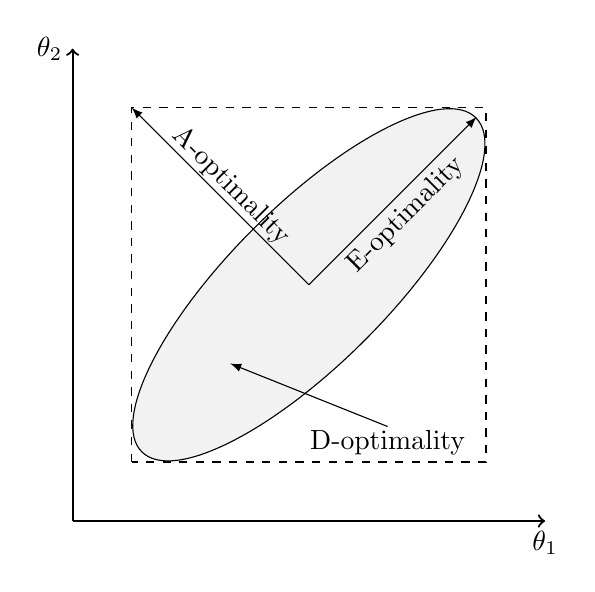
\begin{tikzpicture}
				% Ellipse parameters
				\def\ellipsecenter{(3,3)}
				\def\ellipseA{(0.75,5.25)} % End point for A-optimality arrow
				\def\ellipseB{(5.13,5.13)} % End point for E-optimality arrow
				\def\ellipseC{(4,1.2)}      % End point for D-optimality arrow
				
				% Draw the rotated ellipse
				\draw[fill=gray!10, draw=black, rotate around={45:\ellipsecenter}] \ellipsecenter ellipse (3cm and 1cm);
				
				% Draw the dashed rectangle
				\draw[dashed] (0.75,0.75) rectangle (5.25,5.25);
				
				% Draw the arrows and label them with adjustable positions
				\draw [-latex] \ellipsecenter -- \ellipseA node[yshift=-4cm, xshift=2.5cm,rotate around={-45:\ellipsecenter}] {A-optimality};
				\draw [-latex] \ellipsecenter -- \ellipseB node[yshift=0cm, xshift=-3.9cm,rotate around={45:\ellipsecenter}] {E-optimality};
				\draw [-latex] \ellipseC -- (2,2) node[yshift=-1cm, xshift=2cm] {D-optimality};
				
				% Draw axes
				\draw[thick,->] (0,0) -- (6,0) node[below] {$\theta_1$};
				\draw[thick,->] (0,0) -- (0,6) node[left] {$\theta_2$};
			\end{tikzpicture}
		}%
		\caption{Graphical representation of score functions}
		\label{fig:score_fun}
	\end{figure}
	
	\subsubsection{Problem formulation}
	
	Details on the process model can be found in [article 1]. The model's empirical correlations are derived based on laboratory experiments conducted under various but constant operating conditions: $30 - 40^\circ C$, $100 - 200$ bar, and $3.33-6.67 \cdot 10^{-5}$ kg/s. This study employs a model-based design of experiments technique to design an experiment with dynamically changing conditions to improve the precision of the correlation for $D_i$. The decision variables are adjusted every 10 minutes and are kept constant within each interval (piecewise constant controls). These controls have lower and upper bounds that match the validated range of the process model detailed in [article 1]. The sampling time is set to 5 minutes, and the total extraction time is 300 minutes. The standard deviation $\sigma^2$ was estimated to be 0.10. The analysed correlations consist of two independent variables: Reynolds number and mass flow rate. The Reynolds number is a function of fluid thermodynamic properties and velocity, and the fluid density can be affected by temperature or pressure changes. In this work, the decision variables are the inlet temperature $(T^{in})$ and mass flow rate $(F)$, while the pressure is assumed to remain constant. The initial state is considered isothermal, so $T^0 = T^{in}(t=0)$. The optimal design of experiment problem is solved for multiple values of pressure, namely 100, 125, 150, 175 and 200 bar. %The problem formulation is given by Equation \ref{EQ:Formulation_1}.
	
	\begin{comment}
	
	{\footnotesize
	\begin{equation}
		\begin{aligned} 
			&\Xi^* &= \arg &\min_{ T^{in}, F \in \Xi} \int_{t_0}^{t_f} - \ln j_D(\Xi,\dot{x}) dt  \\
			&\text{subject to}
			& \dot{x} &= G(x,t,\Theta;\Xi) \\
			&& t_0&=0\quad~\text{min} \\
			&& t_f&=300~\text{min} \\
			&& T^{0} &= T^{in}(t=0) \\
			&& P(t) & \in \{100, 125, 150, 175, 200\}~\text{bar} \\
			%&& \dot{y} = g(x(t)) \\
			&& 30^\circ C \leq &T^{in}(t) \leq 40^\circ C \\
			&& 3.33 \cdot 10^{-5} \leq &F(t) \leq 6.67 \cdot 10^{-5}
		\end{aligned} \label{EQ:Formulation_1}
	\end{equation} } 

	\end{comment}

	%The analysed correlation depends on the mass flow-rate and the Reynolds number, which suggest that using a mass-flow rate as an decision variable allow to investigate the whole correlation. Following the general formulation of many control problems such as Linear Quadratic Regulator, a quadratic penalty term is introduced to the cost function to avoid overuse of the mass-flow rate. The penalty term increase the value of the objective function in case of rapid changes of the mass flow-rate. 

	In a real system, the mass flow rate and inlet temperature cannot be changed instantaneously, as they depend on the dynamics of the pump and heat exchanger, respectively. To prevent bang-bang-like control between the lower and upper bounds of the decision variables, a penalty term is introduced. Similar to many control problems, such as the Linear Quadratic Regulator, a quadratic penalty term is added to the cost function. This penalty increases the cost function value when there are rapid changes in the decision variables. The matrix $R$ represents the control cost matrix, with its entries chosen so that the control costs are one order of magnitude lower than $-\ln j_D$. The problem formulation is given by Equation \ref{EQ:Formulation_2}.
	
	{\footnotesize
		\begin{equation}
			\begin{aligned} 
				&\Xi^* &= \arg &\min_{ T^{in}, F \in \Xi} \int_{t_0}^{t_f} - \ln j_D(\Xi,\dot{x}) + u(t) R u(t)^\top dt  \\
				&\text{subject to}
				& \dot{x} &= G(x,t,\Theta;\Xi) \\
				&& t_0&=0\quad~\text{min} \\
				&& t_f&=300~\text{min} \\
				&& T^{0} &= T^{in}(t=0) \\
				&& P(t) & \in \{100, 125, 150, 175, 200\}~\text{bar} \\
				&& R &= \begin{bmatrix}
						10^{-1} & 0  \\
						0 & 10^{-2}
					\end{bmatrix}  \\
				&& u(t) &= \begin{bmatrix}
					\frac{dF(t)}{dt}  \\
					\frac{dT^{in}(t)}{dt} 
				\end{bmatrix}  \\
				%&& \dot{y} = g(x(t)) \\
				&& 30^\circ C \leq &T^{in}(t) \leq 40^\circ C \\
				&& 3.33 \cdot 10^{-5} \leq &F(t) \leq 6.67 \cdot 10^{-5}
			\end{aligned} \label{EQ:Formulation_2}
	\end{equation} } 

\end{document}













































